\chapter{Contexte et présentation}
	\section{Présentation du contexte}

		Créée en 2006, Equida est une société spécialisée dans la vente aux enchères de chevaux de course. Avec un effectif de vingt-sept personnes, la société a réalisé, en 2012, un chiffre d’affaire de 87 millions d’euros. Ses clients sont des vendeurs de chevaux, principalement des haras, des entraîneurs et de grands propriétaires de chevaux, situés en France et à l’étranger. Pour être plus proche de sa clientèle étrangère, elle s’appuie sur une quinzaine de correspondants répartis dans de nombreux pays comme l’Irlande, la Turquie, ou encore le Japon.\newline
		Pour gérer son activité, la société utilise un site web qui permet notamment la consultation des ventes, une application Planning qui permet de gérer les clients, une application de gestion des ventes aux enchères ainsi qu'une application de gestion des informations des chevaux.\newline
		Equida souhaite combiner ses différentes applications en une seule, ce qui lui permettra donc de gérer les chevaux et leurs informations, leurs mises en vente, leurs enchères ainsi que les clients et leur compte.\newline
		Cette application combine des fonctionnalités pour les clients (enregistrement d'un cheval, proposition d'un cheval à une vente, ...) et des fonctionnalités pour l'administrateur (gestion des clients et de leur compte, validation des propositions, ajout de ventes, ...), elle devra contenir deux niveaux d'authentification.\newline
		Pour plus d'informations, vous pouvez consulter la totalité du \href{https://github.com/jmartin-pro/Equida/blob/master/doc/Cahier%20des%20charges.pdf}{cahier des charges}.

		\noindent
		On a fait le choix de réaliser un seul projet contenant deux applications : une application web (voir \nameref{chapter:app_web}) et une application mobile (voir \nameref{chapter:app_mobile}) qui utilisera une api. L'application web est plus complète car destinée à être utiliser surtout par l'administrateur ; l'application mobile, elle, se concentre surtout sur des fonctionnalités propre à l'utilisateur avec tout de même quelques possibilités de gestion pour l'administrateur.

	\section{Choix techno}

		\subsection{MySql}

			MySql, en comparaison avec Oracle, est open source et gratuit. Ce qui le rend avantageux. \newline
			De plus, le cahier des charges fourni par le client retenait la solution de MySql pour la base de données.

		\subsection{Spring Boot}

			On fait le choix de Spring Boot pour le projet car c'est, très probablement, le framework Java pour le développement web le plus utilisé. \newline
			Il permet de créer facilement un contrôleur, en effet, il suffit de créer une classe et de l’annoter @Controller. Les méthodes auront l’annotation @GetMapping, @PostMapping ou pour toute autre méthode HTTP, l'annotation suivant le modèle @XMapping, qui indique l'URL de la page, ainsi que la méthode HTTP, qui lui correspond.\newline
			De plus, il embarque l'équivalent d'un serveur TomCat lors de la compilation du projet (en faisant Tasks > boot > bootRun sur netbeans ou gradle bootRun en ligne de commande) qui permet le démarrage du projet par l'intermédiaire du serveur web embarqué. \newline

			\noindent
			Vous pouvez retrouver ce framework \href{https://spring.io/projects/spring-boot}{ici} ainsi que des tutoriels pour l'utiliser \href{https://www.tutorialspoint.com/spring_boot/index.htm}{ici} et \href{https://www.javatpoint.com/spring-boot-tutorial}{là}.

		\subsection{Ionic}

			Ionic est un framework open source qui permet de créer des applications multiplateformes (mobile et navigateur) performantes tout en utilisant des technologies web connues (HTML, CSS, JavaScript). Il possède en plus une intégration d'Angular qui permet d'appréhender une page web comme un assemblage de composants webs indépendants mais qui peuvent communiquer entre eux. \newline
			Ionic intègre également des composants visuels natifs, ainsi, les utilisateurs d'Android ou d'iOs conserveront leurs habitudes sur l'application. \newline
			Vous pouvez retrouver ce framework \href{https://ionicframework.com/docs/installation/cli}{ici} avec sa documentation \href{https://ionicframework.com/docs/components}{là}.

		\subsection{Gradle}

			Gradle est un "build automation system" (moteur de production). Il est un équivalent plus récent et plus complet à Maven. Il possède de meilleures performances, un bon support pour de nombreux IDE et permet d'utiliser de nombreux dépots, dont ceux de Maven.

	\section{Organisation du projet}
		\subsection{Git et branches}
			On utilise donc Git comme logiciel de gestion de versions, ce qui nous permet de travailler en parallèle sur les mêmes fichiers et d'effectuer chacunes les modifications qui nous concernent sans gêner le travail de l'autre.
			\subsubsection{Branches}

				Afin d'utiliser au mieux Git, nous avons fait le choix de créer deux branches "principales". Il s'agit donc de \textit{master} et de \textit{develop}.\newline
				La branche \textit{master} correspond à la version en production de nos applications. Ainsi, on ne travaillera jamais sur cette branche. Elle ne nous servira donc qu'à récupérer l'application dans un état stable afin d'y mettre les différentes applications en production.\newline
				La branche \textit{develop}, quant à elle, est donc la branche à partir de laquelle nous travaillons. C'est à partir de cette dernière que nous créerons les différentes branches pour le développement de nos fonctionnalités. Ne sont poussées sur celle-ci que les nouvelles fonctionnalités opérationnelles des applications. C'est donc la version en cours de développement.\newline
				Les branches créées à partir de \textit{develop} sont donc les branches correspondant aux fonctionnalités développées, elles commencent toutes par features/XXX (correspondant à la modification). Par exemple, pour la gestion des clients, on crera une branche features/gestionClients.

			\subsubsection{Nomenclature}

				Pour une meilleure homogénéisation de la gestion des versions, on choisit d'établir et d'utiliser une nomenclature pour les messages de commit. Cette nomenclature est consultable dans le fichier CONVENTIONS.md.\newline
				On y retrouve notamment les commits pour l'ajout de fonctionnalités sous le nom de  \textit{feat}, pour les corrections de bug  \textit{fix}, pour la documentation  \textit{doc}, ...
				Ce qui donne des messages comme celui-ci :  \textit{feat : Ajout de la modification d'un client}.


		\subsection{Les différents dossiers}
			\subsubsection{Doc}

				On a fait le choix de rédiger la documentation du projet avec Latex car c'est un système de création de documents opensource. De plus, les fichiers Latex sont facilement gérés par Git contrairement aux fichiers Word. On peut ainsi manipuler aisément les différentes versions des documents. Il permet également une compilation directe au format pdf.

			\subsubsection{SQL}

			Les fichiers SQL (situés dans le dossier  \textit{/sql}) sont donc ceux qui vont créer la base de données. Il suffit d'importer les scripts dans l'ordre afin de la restituer. On nomme les fichiers précédés d'un numéro (ordre d'importation) suivi de l'intitulité de la modification. Les tables de la BDD sont en majuscules séparéés par des underscore si besoin tandis que les champs respectent la norme CamelCase.

			\subsubsection{Sources}

				Dans le dossier source, on retrouve donc deux sous-dossiers : un sous-dossier ionic et un Spring.
				Le sous-dossier ionic, comme son nom le suggère, correspond au code prore à l'application mobile (développée avec Ionic). On retrouvera donc à l'intérieur, des fichiers json, html, service.ts. On reviendra plus en détail sur cette partie par la suite.
				Le sous-dossier Spring, correpondant à SpringBoot, contient, quant à lui, les dossiers core, gradle, rest et webApp. Ces derniers comprennent notamment et respectivement les fichiers communs aux deux applications (bdd, service...), les fichiers de configuration, le code de l'API ainsi que le code de l'application web (controller, routes, formulaires, ...).

		\subsection{Trello}

			Le planning, la répartition des tâches et le fonctionnement du projet sont visibles sur le \href{https://trello.com/b/jrKixhpu/equida-spring}{Trello}.
			Pensez à consulter les cartes archivées pour voir le travail effectué. En effet, les modifications effectuées sont archivées afin de ne pas les conserver dans les activités à faire ou en cours.

	\section{Intéractions entre les différentes parties du projet}
		\subsection{Les différentes parties}
			Le projet Équida est composé de 2 applications. Une application web, qui est également l'application principale et une application mobile qui est à l'usage principal des clients. Les 2 applications s'appuient sur la même \bdd{}. L'application web y est directement connectée. L'application mobile, elle, passe par une API. En effet, si celle-ci se connectait directement à la \bdd{}, comme c'est le cas pour l'application web, une personne mal intentionnée serait en mesure de décompiler l'application mobile et ainsi obtenir les identifiants de la \bdd{}. L'utilisation de cette API empêche donc, notamment, ce problème de sécurité.

			\begin{figure}[H]
				\centering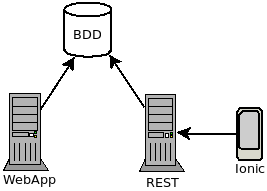
\includegraphics[width=0.45\textwidth, keepaspectratio]{res/diag_infra.png}
				\caption{La connexion à la BDD selon le projet}
			\end{figure}

			L'API ainsi que l'application web utilisent le framework Spring Boot. Ces 2 applications constituent donc 2 projets différents,  \textit{webApp} pour la partie web et  \textit{rest} pour l'API. Ces dernières nécessitant un code identique pour les Services, les Entity et les Repository, nous avons donc fait le choix de créer un projet commun  \textit{core}. On y retrouve donc tout le code commun aux 2 autres projets (cités précédemment mais également les exceptions ou certains outils).

			\begin{figure}[H]
				\centering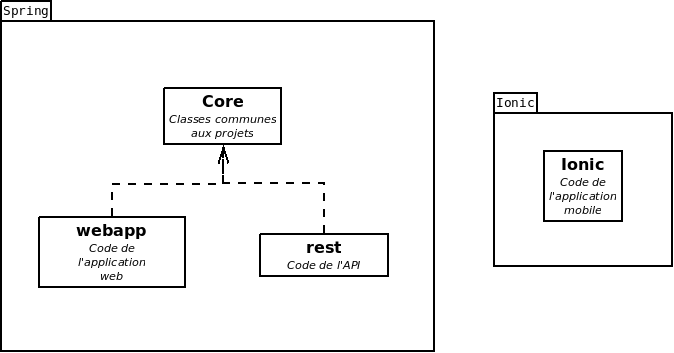
\includegraphics[width=0.75\textwidth, keepaspectratio]{res/diag_projet.png}
				\caption{Les dépendances entre les projets}
			\end{figure}

		\subsection{Configuration Gradle}

			Pour gérer correctement les différents projets basés sur Spring, leurs dépendances ainsi que leurs configurations, nous avons donc utilisé Gradle. Dans le dossier \textit{src/Spring} on retrouve le \textit{build.gradle} qui se charge de configurer la totalité du projet. On peut observer la configuration suivante pour tous.

			\begin{figure}[H]
				\centering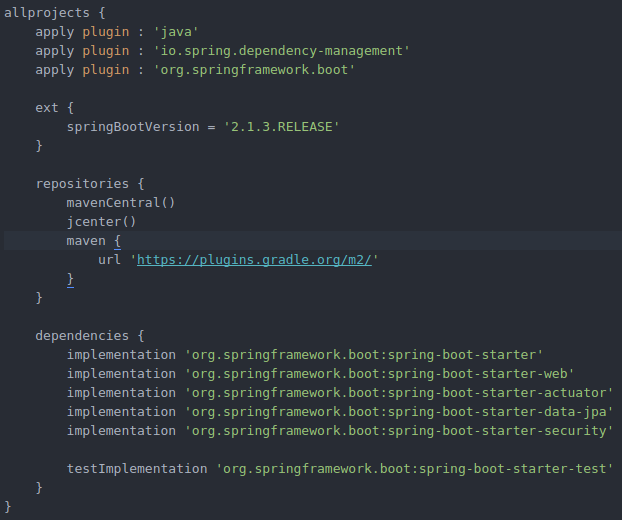
\includegraphics[width=0.75\textwidth, keepaspectratio]{res/gradle_allprojects.png}
				\caption{Configuration Gradle commune à tous les projets}
			\end{figure}

			On précise donc la version de Spring à utiliser, en plus des dépendances communes à tous les projets (spring-boot-starter-web, spring-boot-starter-data-jpa, ...).

			\newpage
			Par la suite, on définit les dépendances uniques à chaque projet.

			\begin{figure}[H]
				\centering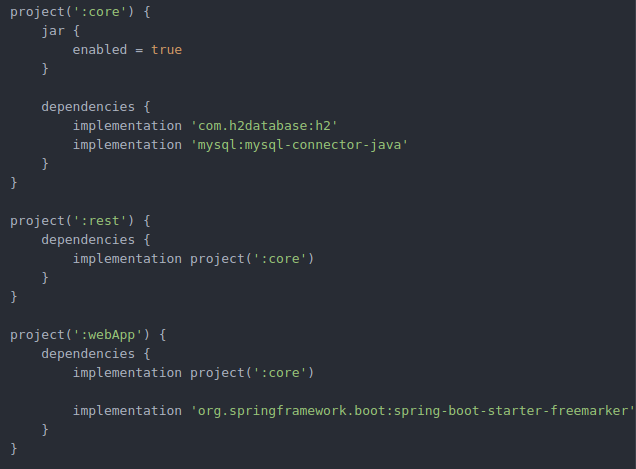
\includegraphics[width=0.75\textwidth, keepaspectratio]{res/gradle_project.png}
				\caption{Configuration Gradle propre à chaque projet}
			\end{figure}

			De même, concernant le projet core, on active uniquement la compilation en jar (comme une librairie) et non pas en jar bootable (comme c'est le cas lorsque l'on utilise Spring Boot).

			\noindent
			D'autres scripts "build.gradle" se trouvent dans chaque dossier du projet, cependant, ceux-ci ne configurent que le nom du projet à l'issue du build, la version du JDK utilisée ainsi que le package de base du projet.
